\documentclass{article} % For LaTeX2e
\usepackage{nips14submit_e,times}
\usepackage{hyperref}
\usepackage{url}
\usepackage{graphicx}
\graphicspath{ {fig/} }
\usepackage{amsmath}
\usepackage{subfigure}
%\documentstyle[nips14submit_09,times,art10]{article} % For LaTeX 2.09


\title{EM Algorithm with Genetic Evolution}


\author{
David S.~Hippocampus\thanks{ Use footnote for providing further information
about author (webpage, alternative address)---\emph{not} for acknowledging
funding agencies.} \\
Department of Computer Science\\
Cranberry-Lemon University\\
Pittsburgh, PA 15213 \\
\texttt{hippo@cs.cranberry-lemon.edu} \\
\And
Coauthor \\
Affiliation \\
Address \\
\texttt{email} \\
\AND
Coauthor \\
Affiliation \\
Address \\
\texttt{email} \\
\And
Coauthor \\
Affiliation \\
Address \\
\texttt{email} \\
\And
Coauthor \\
Affiliation \\
Address \\
\texttt{email} \\
(if needed)\\
}

% The \author macro works with any number of authors. There are two commands
% used to separate the names and addresses of multiple authors: \And and \AND.
%
% Using \And between authors leaves it to \LaTeX{} to determine where to break
% the lines. Using \AND forces a linebreak at that point. So, if \LaTeX{}
% puts 3 of 4 authors names on the first line, and the last on the second
% line, try using \AND instead of \And before the third author name.

\newcommand{\fix}{\marginpar{FIX}}
\newcommand{\new}{\marginpar{NEW}}

\nipsfinalcopy % Uncomment for camera-ready version

\begin{document}


\maketitle

\begin{abstract}
The abstract paragraph should be indented 1/2~inch (3~picas) on both left and
right-hand margins. Use 10~point type, with a vertical spacing of 11~points.
The word \textbf{Abstract} must be centered, bold, and in point size 12. Two
line spaces precede the abstract. The abstract must be limited to one
paragraph.
\end{abstract}

%%%%%%%%%%%%%%%%%%%%%%%%%%%%%%%%%%%%%%%%%%%%%%%%%%%%%%%%%%%%%%%%%%%%%%%%%%%%%
\section{Introduction}
%%%%%%%%%%%%%%%%%%%%%%%%%%%%%%%%%%%%%%%%%%%%%%%%%%%%%%%%%%%%%%%%%%%%%%%%%%%%%

\subsection{Motivation}

\subsection{Genetic algorithm}


%%%%%%%%%%%%%%%%%%%%%%%%%%%%%%%%%%%%%%%%%%%%%%%%%%%%%%%%%%%%%%%%%%%%%%%%%%%%%
\section{Method: genetic-based EM algorithm (GA-EM)}
%%%%%%%%%%%%%%%%%%%%%%%%%%%%%%%%%%%%%%%%%%%%%%%%%%%%%%%%%%%%%%%%%%%%%%%%%%%%%

\subsection{Model selection criterion: MDL}

\subsection{Encoding}

Each individual in the population is composed of three parts, as shown in Figure~\ref{fig:encoding}. The first part (Part A) uses binary encoding, where the total number of bits is determined by the maximal number of allowed components $M_{\max}$. Each bit represents one particular Gaussian component in the model. If the bit is set to 0, then its associated component is omitted for modeling the mixture. In contrast, if the bit is set to 1, then it means this component is responsible for some data points in the mixture. The second part (Part B) uses floating point value encoding to record the components weight $\mathbf{w}$ of which the length is $M_{\max}$. Note that due to the switching mechanism of the components among individuals during evolution, the weight might need to be reset to uniform distribution except for the best individual (elitist). And the principle is to keep the weight as long as possible. The third part (Part C) also uses floating point value encoding to record the mean $\boldsymbol{\mu_m}$ and covariance $\boldsymbol{\Sigma_m}$ (and maybe other parameters) of the $M_{\max}$ components. 


\begin{figure}[h]
\begin{center}
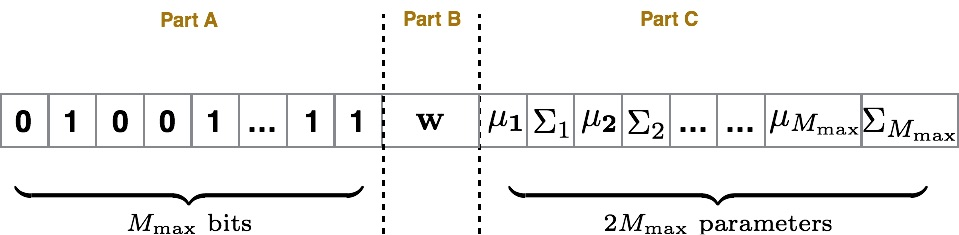
\includegraphics[scale=0.3]{encoding.jpg}
\end{center}
\caption{Encoding of individuals.}
\label{fig:encoding}
\end{figure}

 
\subsection{Recombination}

The crossover operator selects two parent individuals randomly from the current population $\mathbf{P}$ and recombines them to form two offsprings. Total number of $H$ ($H<K$ and is a multiple of 2) children will be generated in this step. We use \textit{single-point crossover} (\textbf{TOCITE}), which chooses randomly a cross-over position $\chi = \{1, \ldots, M_{\max}\}$ within Part A of the individual and exchanges the value of the genes to the right of this position between two selected parent individuals, as shown in Figure~\ref{fig:recombination}. Part B of the offsprings are set to uniform distribution and Part C are exchanged correspondingly.

\begin{figure}[h]
\begin{center}
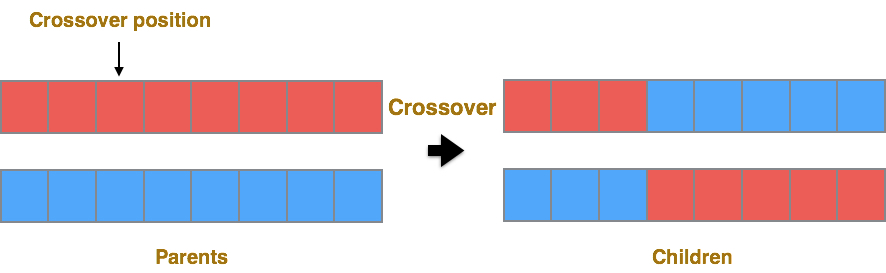
\includegraphics[scale=0.3]{recombination.jpg}
\end{center}
\caption{Recombination: single-point crossover.}
\label{fig:recombination}
\end{figure}

\subsection{Selection}

\subsection{Enforced mutation}

\subsection{Mutation}

\subsection{Implementation}



%%%%%%%%%%%%%%%%%%%%%%%%%%%%%%%%%%%%%%%%%%%%%%%%%%%%%%%%%%%%%%%%%%%%%%%%%%%%%
\section{Results and Discussion}
%%%%%%%%%%%%%%%%%%%%%%%%%%%%%%%%%%%%%%%%%%%%%%%%%%%%%%%%%%%%%%%%%%%%%%%%%%%%%

\subsection{Initialization}

The start population $\mathbf{P^0}$ is composed of a set of $K$ individuals, where each individual has randomly selected $M$ components. We explored two initialization methods:
\begin{enumerate}
\item \textit{random}: The mean values of each component $\boldsymbol{\mu^0_m}$ are set to randomly selected data points. The covariance matrices $\boldsymbol{\Sigma^0_m}$ are initialized as the sample covariance matrix of all data. The weights $\mathbf{w^0_m}$ of the components are assumed to be uniformly distributed.
\item \textit{k-means}: The parameters of the selected components are initialized by the k-means algorithm with $k=M$. The mean values of each component $\boldsymbol{\mu^0_m}$ are set to the cluster centroids. The covariance matrices $\boldsymbol{\Sigma^0_m}$ are initialized to the sample covariance matrices of the data in the corresponding cluster. The weights $\mathbf{w^0_m}$ of the components are the responsibilities of each cluster.
\end{enumerate}

We have explored the influence of these two initialization methods, as shown in Figure~\ref{fig:init}. We added EM runs with the right number of component using two initialization for comparison. Note that the iteration numbers of the EM runs were scaled to accommodate the GA-EM runs. We observe that there are no significant performance difference on the two initialization.
\begin{figure}[htp]
  \begin{center}
    \subfigure[]{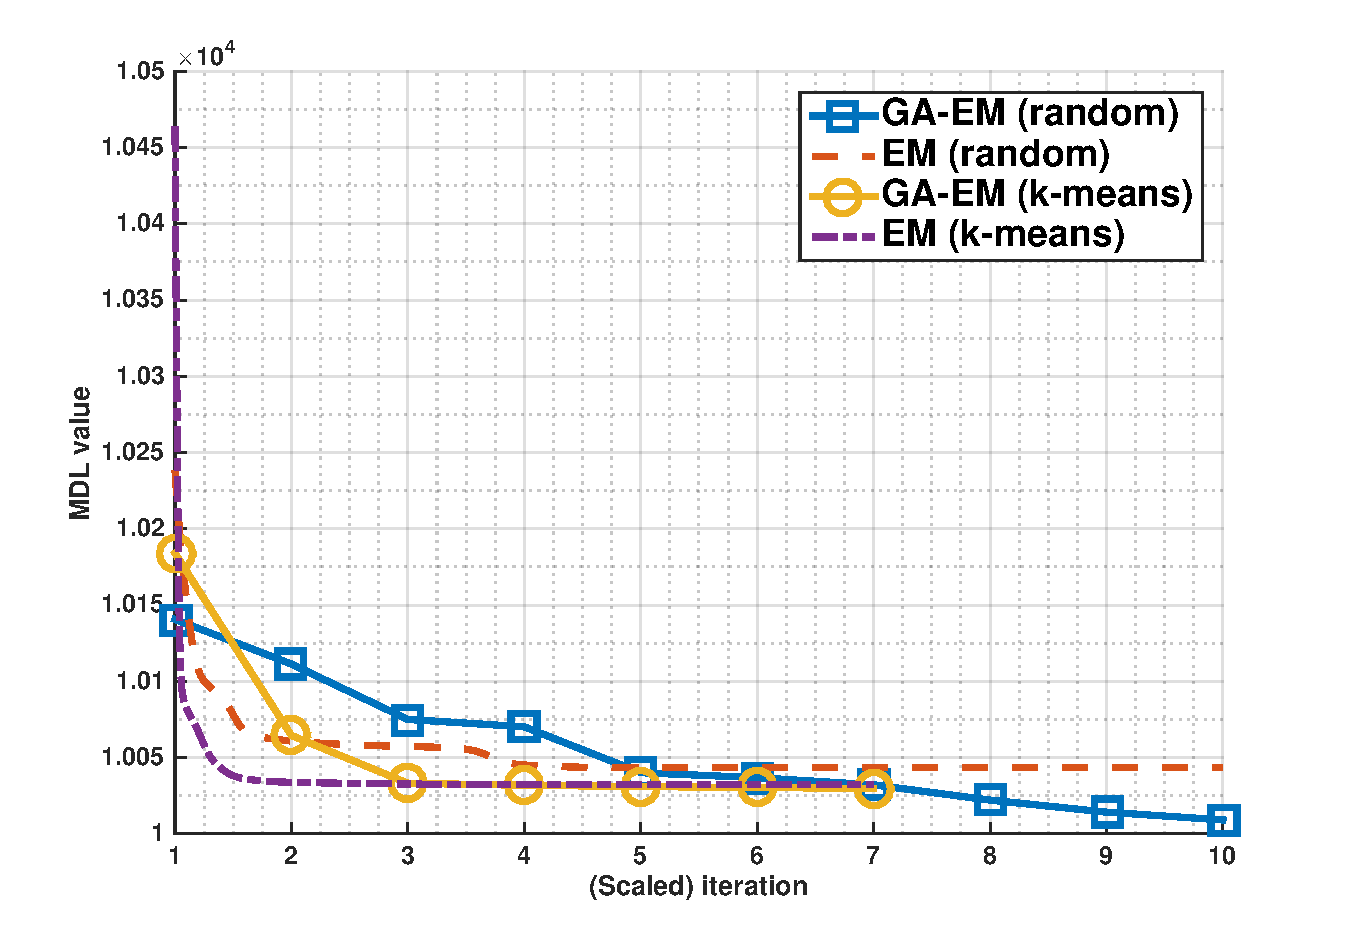
\includegraphics[width=6.8cm]{init_syn_1.pdf}}
    \subfigure[]{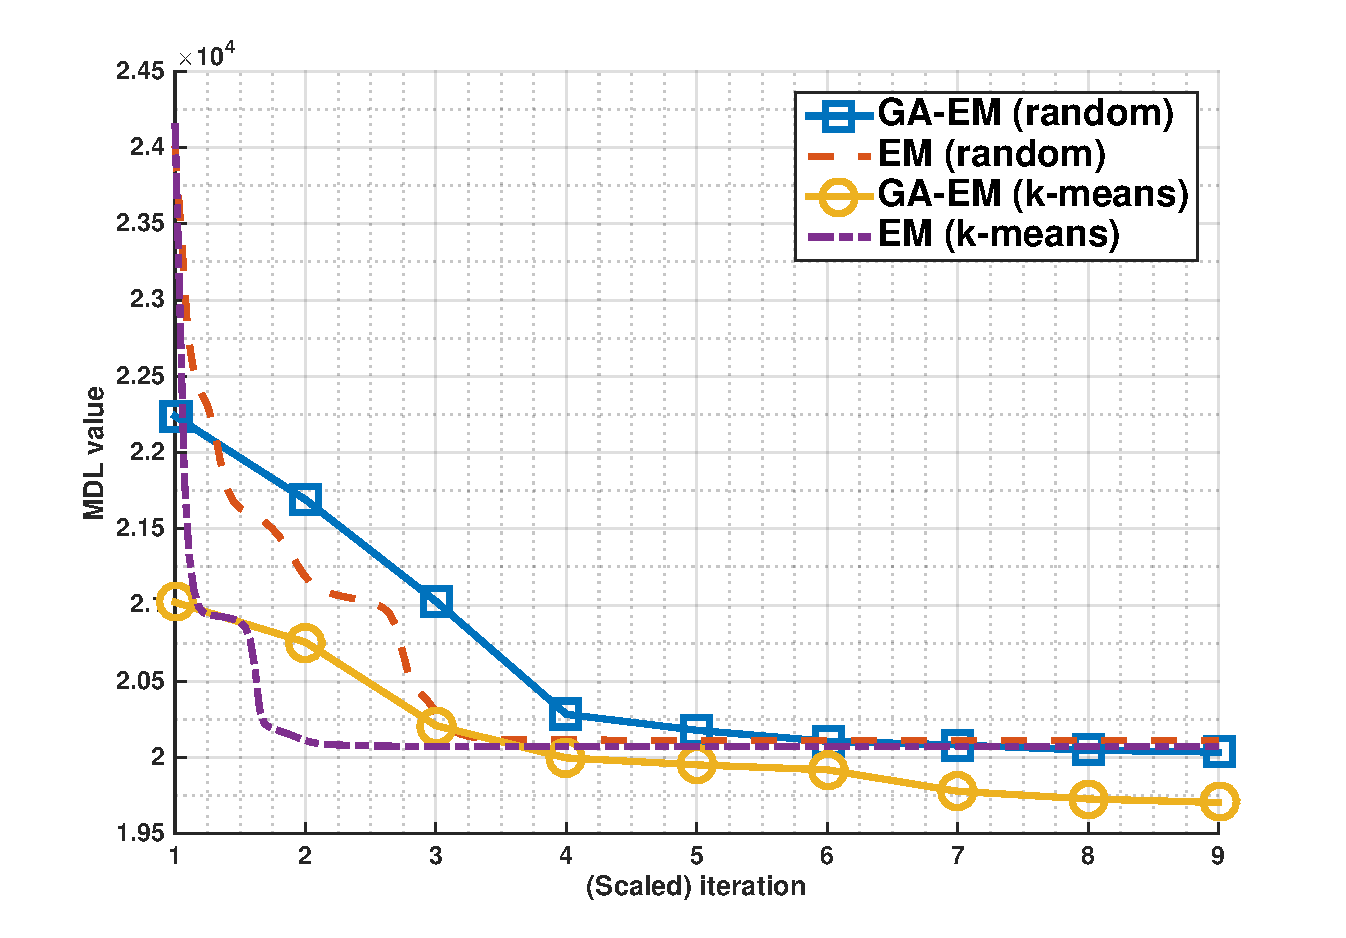
\includegraphics[width=6.8cm]{init_penpca_1.pdf}}
  \end{center}
  \caption{Influence of initialization on GA-EM and EM algorithms. (a) Simulated data. (b) PCA transformed Pendigit data.}
  \label{fig:init}
\end{figure}

\subsection{Model selection}

There are several parameters in the GA-EM algorithm to be determined to guarantee the performance. We have run the algorithm on both simulated data (Figure~\ref{fig:mod_sel_syn}) and real PCA transformed Pendigit data (Figure~\ref{fig:mod_sel_penpca}).

\begin{itemize}
\item $R$: number of EM steps executed in the population. It stops impacting the convergence of the algorithm after $R$ goes beyond $10$. We set $R=10$.
\item $K$: population size. It in general shows negligible effect on the behavior. We set $K=6$.
\item $H$: number of offsprings generated. Here we used $K = 20$. It shows no significant effect on the behavior. We set $H=4$.
\item $M_{\max}$: maximal number of allowed components in each individual. It shows analogy behavior for $M_{\max} \geq 15$. We set $M_{\max} = 20$.
\item $p_m$: mutation probability. It shows negligible effect on the behavior. We set $p_m=0.1$.
\item $t_{corr}$: correlation threshold. It shows negligible effect on the behavior except for very low correlation values. We set $t_{corr}=0.95$.
\end{itemize}

\begin{figure}[h]
\begin{center}
\makebox[\textwidth][c]{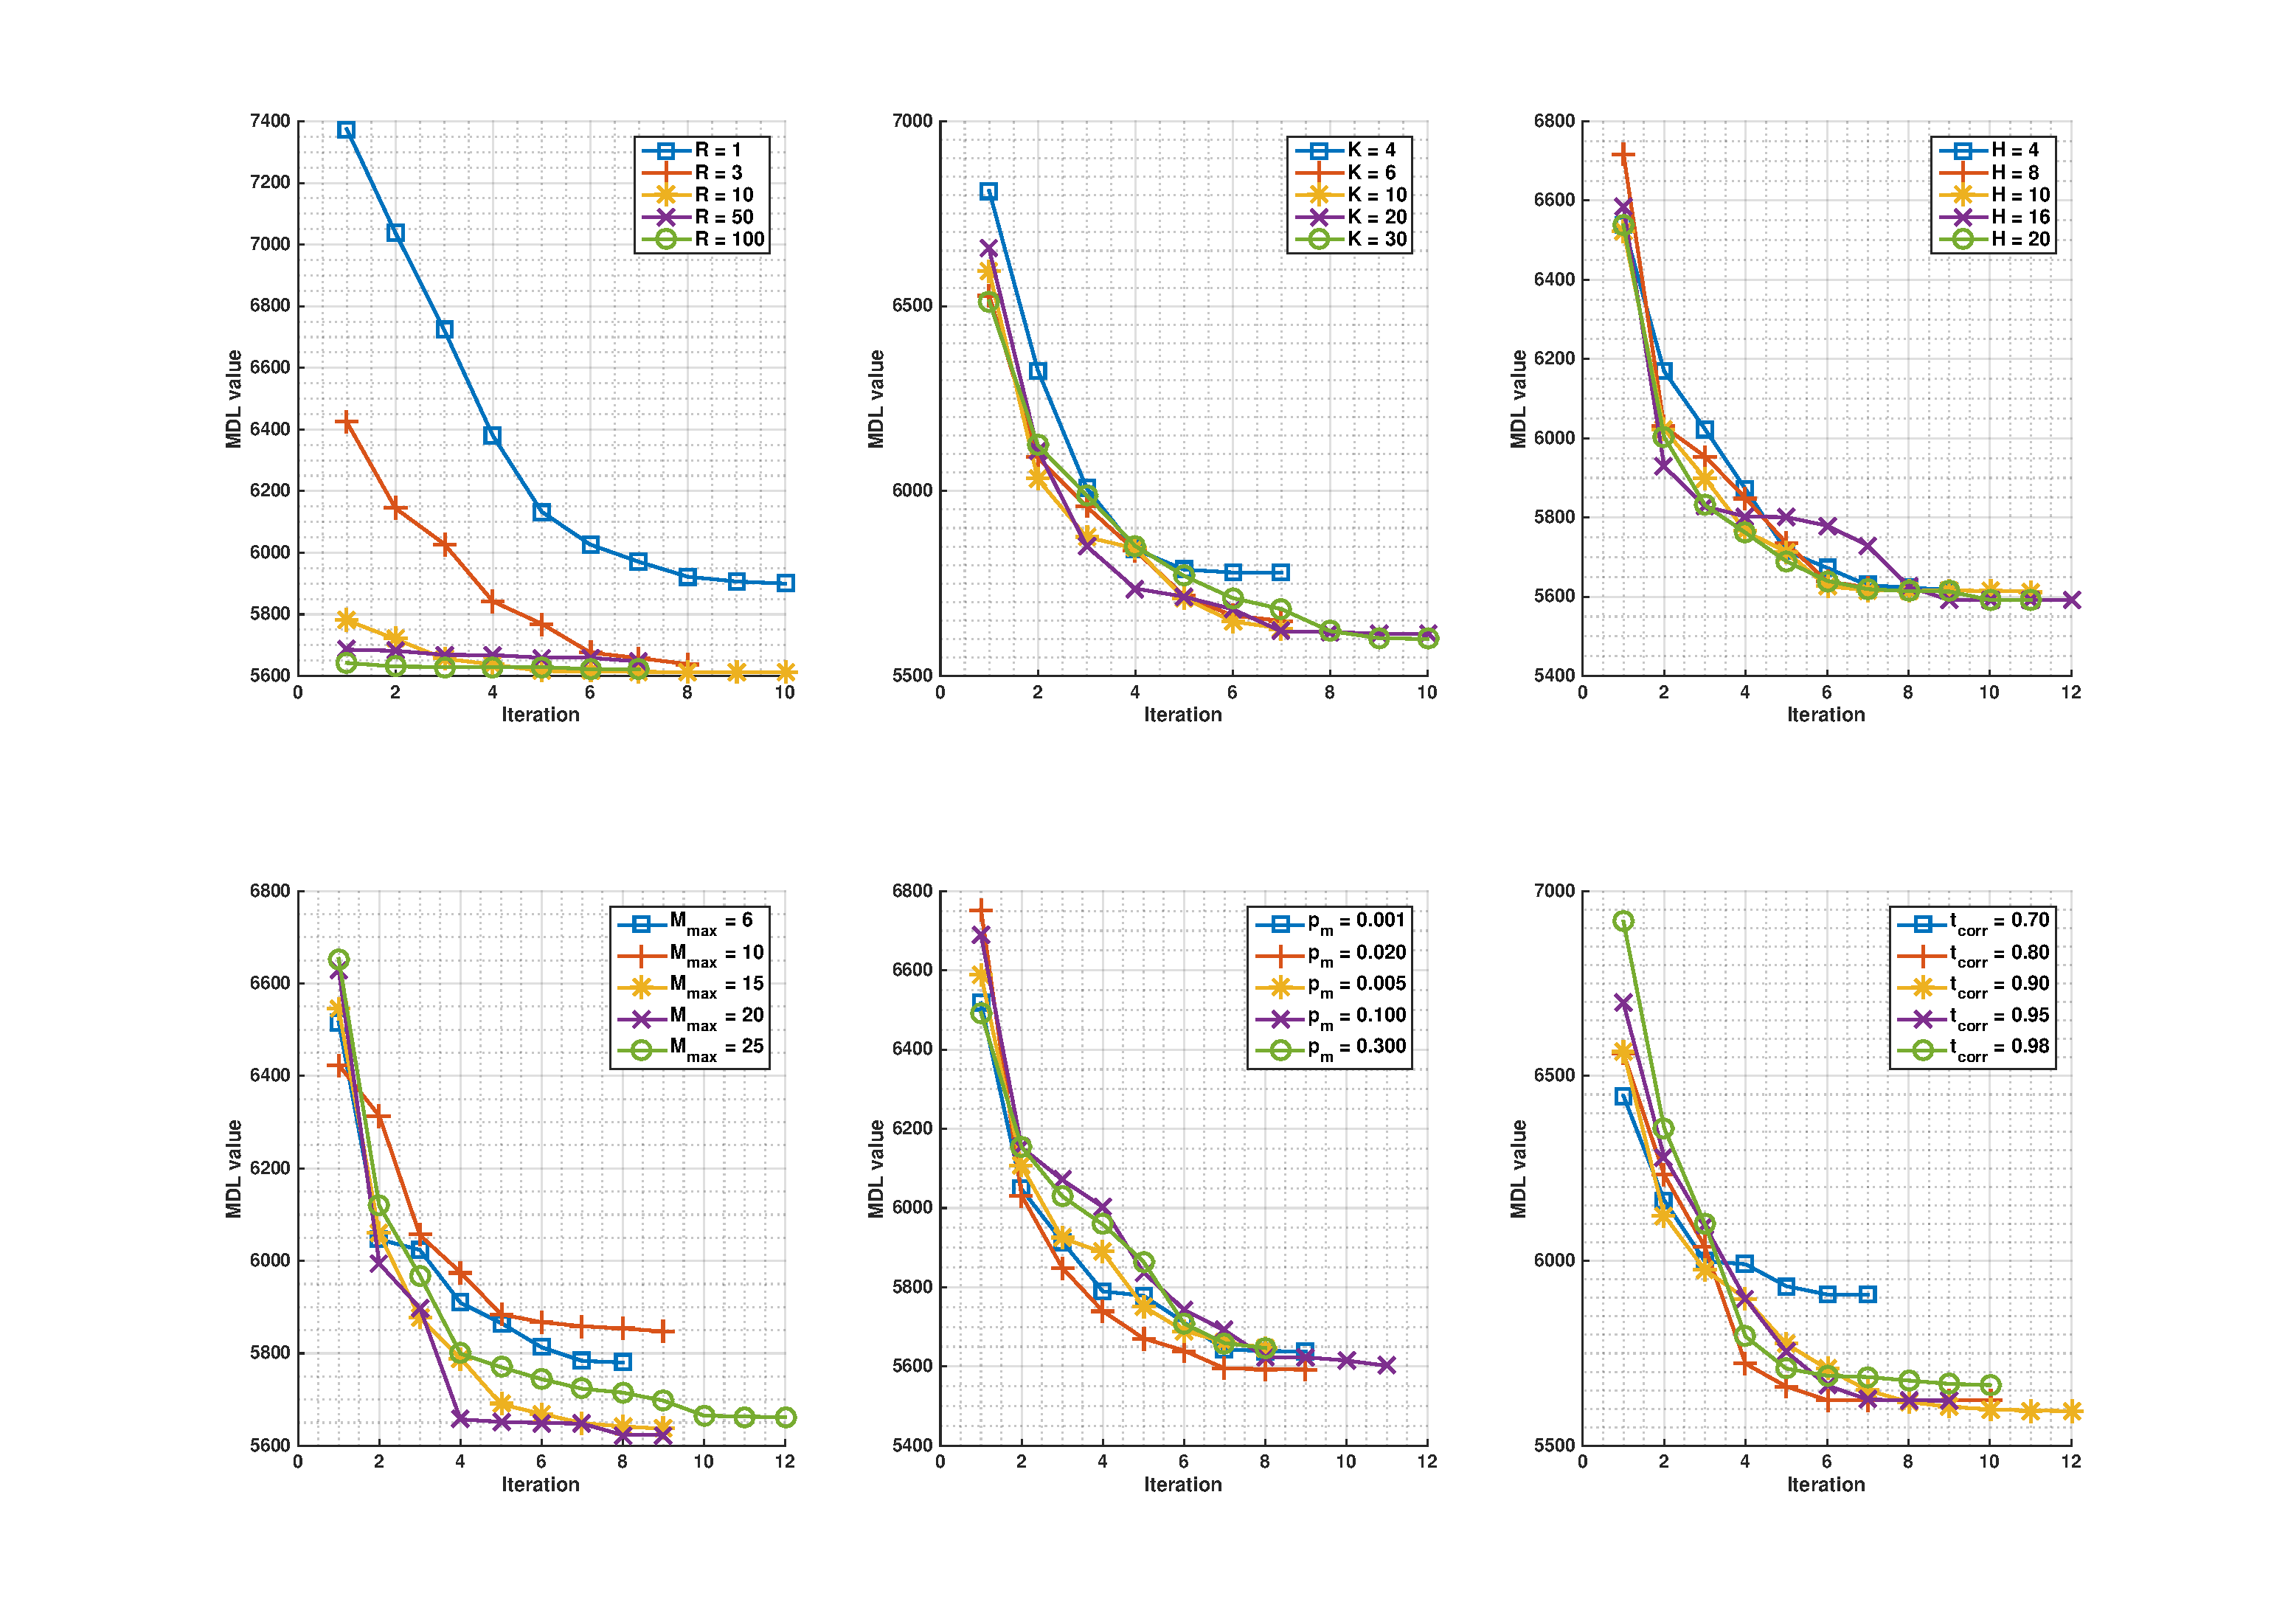
\includegraphics[scale=0.4]{model_sel_syn_1.pdf}}
\end{center}
\caption{Influence of parameters on GA-EM algorithm with simulated data.}
\label{fig:mod_sel_syn}
\end{figure}

\begin{figure}[h]
\begin{center}
\makebox[\textwidth][c]{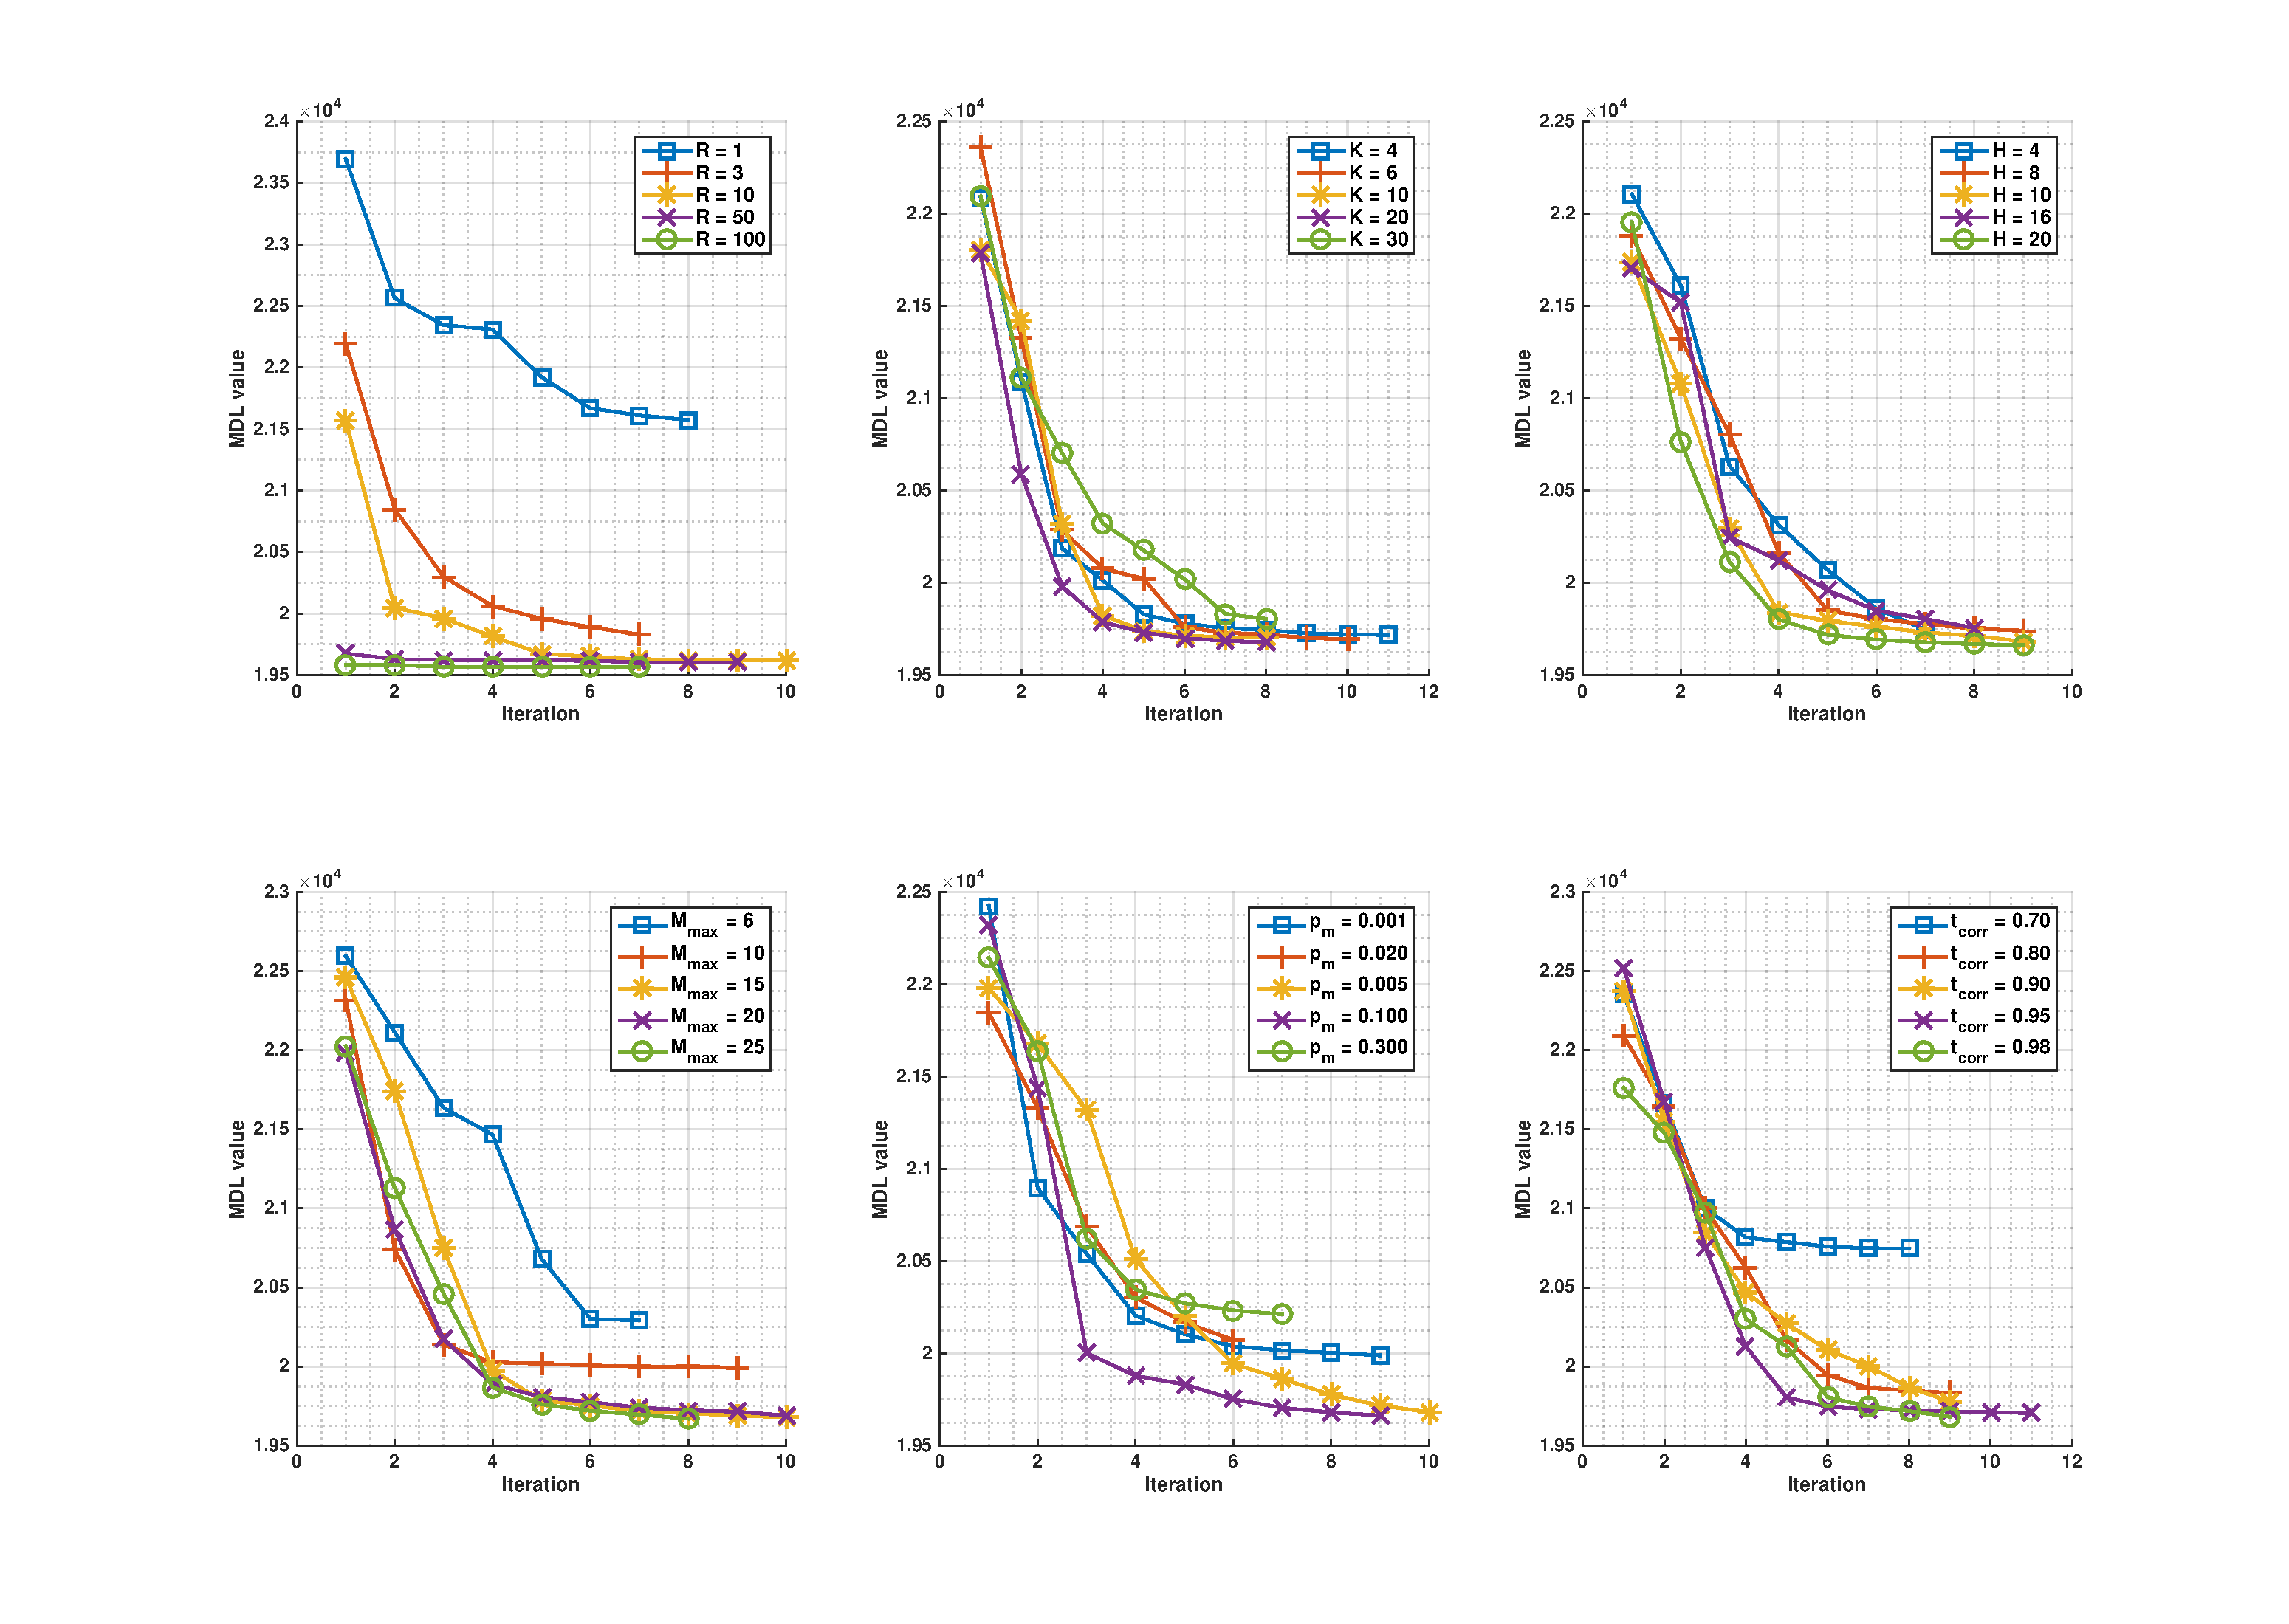
\includegraphics[scale=0.4]{model_sel_penpca_1.pdf}}
\end{center}
\caption{Influence of parameters on GA-EM algorithm with PCA transformed Pendigit data.}
\label{fig:mod_sel_penpca}
\end{figure}
 
\subsection{Application on real data}

\subsection{Performance}

\subsection{Extension of GA-EM}


%%%%%%%%%%%%%%%%%%%%%%%%%%%%%%%%%%%%%%%%%%%%%%%%%%%%%%%%%%%%%%%%%%%%%%%%%%%%%
\section{Summary and future work}
%%%%%%%%%%%%%%%%%%%%%%%%%%%%%%%%%%%%%%%%%%%%%%%%%%%%%%%%%%%%%%%%%%%%%%%%%%%%%




\subsubsection*{Acknowledgments}

Use unnumbered third level headings for the acknowledgments. All
acknowledgments go at the end of the paper. Do not include 
acknowledgments in the anonymized submission, only in the 
final paper. 

\subsubsection*{References}

References follow the acknowledgments. Use unnumbered third level heading for
the references. Any choice of citation style is acceptable as long as you are
consistent. It is permissible to reduce the font size to `small' (9-point) 
when listing the references. {\bf Remember that this year you can use
a ninth page as long as it contains \emph{only} cited references.}

\small{
[1] Alexander, J.A. \& Mozer, M.C. (1995) Template-based algorithms
for connectionist rule extraction. In G. Tesauro, D. S. Touretzky
and T.K. Leen (eds.), {\it Advances in Neural Information Processing
Systems 7}, pp. 609-616. Cambridge, MA: MIT Press.

[2] Bower, J.M. \& Beeman, D. (1995) {\it The Book of GENESIS: Exploring
Realistic Neural Models with the GEneral NEural SImulation System.}
New York: TELOS/Springer-Verlag.

[3] Hasselmo, M.E., Schnell, E. \& Barkai, E. (1995) Dynamics of learning
and recall at excitatory recurrent synapses and cholinergic modulation
in rat hippocampal region CA3. {\it Journal of Neuroscience}
{\bf 15}(7):5249-5262.
}

\end{document}
